\section{Experimental results}
\label{sec:experiments}

\subsection{Arithmetic datasets}
\label{sec:arithmetic-dataset}

The arithmetic dataset is a replica of the "simple function task" as shown in \cite{trask-nalu}.
The goal is to sum two random subsets of a vector and perform a arithmetic operation as defined below
\begin{equation}
t = \sum_{i = s_{1,\mathrm{start}}}^{s_{1,\mathrm{end}}} x_i \circ \sum_{i = s_{2,\mathrm{start}}}^{s_{2,\mathrm{end}}} x_i \quad \text{where } \mathbf{x} \in \mathbb{R}^n, x_i \sim \mathrm{Uniform}[r_{\mathrm{lower}}, r_{\mathrm{upper}}], \circ \in \{+, -, \times\}
\label{eq:arithmetic-problem}
\end{equation}
where $n$ (default $100$), $U[r_{\mathrm{lower}}, r_{\mathrm{upper}}]$ (interpolation default is $U[1,2]$ and extrapolation default is $U[2,6]$), $\circ$, the subset size (default 25\%), and subset overlap (default 50\%) are dataset parameters that we use to assess learning capability (see details in appendix \ref{sec:appendix:simple-function-task:data-generation} and the effect of these parameters in appendix \ref{sec:appendix-simple-function-task:dataset-parameter-effect}).

\subsubsection{Model evaluation}
The goal is to achieve a solution that is acceptably close to a perfect solution. To evaluate if a model instance solves the task consistently we compare the MSE to a nearly-perfect solution on the extrapolation range over multiple seeds. If $\mathbf{W}_1, \mathbf{W}_2$ defines the weights of the fitted model, and $\mathbf{W}_1^\epsilon$ is nearly-perfect and $\mathbf{W}_2^*$ is perfect (example in equation \ref{eq:nearly-perfect-solution-example}), the success criteria is $\mathcal{L}_{\mathbf{W}_1, \mathbf{W}_2} < \mathcal{L}_{\mathbf{W}_1^\epsilon, \mathbf{W}_2^*}$, measured on the extrapolation error, for $\epsilon = 10^{-5}$.
\begin{equation}
    \mathbf{W}_1^\epsilon = \begin{bmatrix}
    1 - \epsilon & 1 - \epsilon & 0 + \epsilon & 0 + \epsilon \\
    1 - \epsilon & 1 - \epsilon & 1 - \epsilon & 1 - \epsilon
    \end{bmatrix}, \mathbf{W}_2^* = \begin{bmatrix}
    1 & 1
    \end{bmatrix}
    \label{eq:nearly-perfect-solution-example}
\end{equation}
To measure speed of convergence the first iteration for which $\mathcal{L}_{\mathbf{W}_1, \mathbf{W}_2} < \mathcal{L}_{\mathbf{W}_1^\epsilon, \mathbf{W}_2^*}$ is reported with a 95\% confidence interval. Only models that managed to solve the task are considered.

We assume an approximate discrete solution with parameters close to $\{-1, 0, 1\}$ is important for inferring exact arithmetic operations.
To measure the sparsity we introduce a sparsity error (defined in equation \ref{eq:sparsity-error}).
Similar to the convergence metric we only considered model instances that did solve the task and report the 95\% confidence interval.
\begin{equation}
E_\mathrm{sparsity} = \max_{h_{\ell-1}, h_{\ell}} \min(|W_{h_{\ell-1},h_\ell}|, |1 - |W_{h_{\ell-1},h_\ell}||)
\label{eq:sparsity-error}
\end{equation}

We evaluate each metric every $1000$ iterations based on the test set that uses the extrapolation range, and choose the best iteration based on the validation dataset that uses the interpolation range.

%\subsubsection{Experimental setup}

%The multiplication models, NMU and $\mathrm{NAC}_{\bullet}$, have an addition layer first, either NAU or $\mathrm{NAC}_{+}$, followed by a multiplication layer. The addition models, $\mathrm{NAC}_{+}$, NAU, and Linear are just two layers of that unit. Finally, the NALU model consists of two NALU layers. See explicit definitions in appendix \ref{sec:appendix:comparison-all-models}.% All models are fitted with an mean-squared-error loss-function.

%For all experiments $\lambda_{\mathrm{sparse}} = \max(\min(\frac{t - \lambda_{\mathrm{start}}}{\lambda_{\mathrm{end}} - \lambda_{\mathrm{start}}}, 1), 0)$. The motivation here, is that the optimization consists of two parts. A warmup period, where $W_{h_{\ell-1},h_\ell}$ should get close to the solution, unhindered by the sparsity regualizer, and then a finalize period where the solution is made sparse. We show the effect of regularization in appendix \ref{sec:appendix:simple-function-task:regualization}.% All models are optimized with Adam optimization \cite{adam-optimization} using default parameters and trained for about four hours on an HPC cluster running \text{8-Core Intel Xeon E5-2665 2.4GHz} CPUs.

%The training dataset is continuously sampled from the interpolation range where a different seed is used for each experiment, all experiments has a mini-batch size of 128 observations, a fixed validationset with $1 \cdot 10^4$ observations sampled from the interpolation range, and a fixed testset with $1 \cdot 10^4$ observations sampled from the extrapolation range.

\subsubsection{Arithmetic operation comparison}
The multiplication models, NMU and $\mathrm{NAC}_{\bullet}$, have an addition layer first, either NAU or $\mathrm{NAC}_{+}$, followed by a multiplication layer. The addition models, $\mathrm{NAC}_{+}$, NAU, and Linear are just two layers of that unit. Finally, the NALU model consists of two NALU layers. See explicit definitions in appendix \ref{sec:appendix:comparison-all-models}.

We compare the models on different arithmetic operation $\circ \in \{+, -, \times\}$, results are seen in table \ref{tab:function-task-static-defaults}, where each experiment is trained for $5 \cdot 10^6$ iterations. Comparison with more models can be found in appendix \ref{sec:appendix:comparison-all-models} and an ablation study of the NMU can be found in appendix \ref{sec:appendix:ablation-study}.

For multiplication, the NMU succeeds more often and converges faster. For addition and subtraction, the NAU model converges faster, given the median, and has a sparser solution.

\begin{table}[!h]

\caption{\label{tab:function-task-static-defaults}Shows the success-rate for $\mathcal{L}_{\mathbf{W}_1, \mathbf{W}_2} < \mathcal{L}_{\mathbf{W}_1^\epsilon, \mathbf{W}_2^*}$, at what global step the model converged at, and the sparsity error for all weight matrices.}
\centering
\begin{tabular}{crllll}
\toprule
\multicolumn{1}{c}{Op} & \multicolumn{1}{c}{Model} & \multicolumn{1}{c}{Success} & \multicolumn{2}{c}{Solved at} & \multicolumn{1}{c}{Sparsity error} \\
\cmidrule(l{3pt}r{3pt}){1-1} \cmidrule(l{3pt}r{3pt}){2-2} \cmidrule(l{3pt}r{3pt}){3-3} \cmidrule(l{3pt}r{3pt}){4-5} \cmidrule(l{3pt}r{3pt}){6-6}
 &  & Rate & Median & Mean & Mean\\
\midrule
 & $\mathrm{NAC}_{\bullet}$ & $30\%$ & $2.5 \cdot 10^{6}$ & $2.5 \cdot 10^{6} \pm 1.5 \cdot 10^{6}$ & $\mathbf{3.9 \cdot 10^{-4} \pm 9.4 \cdot 10^{-4}}$\\

 & Linear & $0\%$ & --- & --- & ---\\

 & NALU & $0\%$ & --- & --- & ---\\

\multirow{-4}{*}{\centering\arraybackslash $\bm{\times}$} & NMU & $\mathbf{90\%}$ & $\mathbf{1.4 \cdot 10^{6}}$ & $\mathbf{1.6 \cdot 10^{6} \pm 5.6 \cdot 10^{5}}$ & $1.8 \cdot 10^{-3} \pm 1.1 \cdot 10^{-3}$\\
\cmidrule{1-6}
 & $\mathrm{NAC}_{+}$ & $\mathbf{100\%}$ & $6.0 \cdot 10^{4}$ & $7.1 \cdot 10^{4} \pm 2.4 \cdot 10^{4}$ & $4.8 \cdot 10^{-1} \pm 2.0 \cdot 10^{-2}$\\

 & Linear & $\mathbf{100\%}$ & $4.2 \cdot 10^{4}$ & $\mathbf{4.2 \cdot 10^{4} \pm 1.9 \cdot 10^{3}}$ & $6.1 \cdot 10^{-1} \pm 1.2 \cdot 10^{-1}$\\

 & NALU & $0\%$ & --- & --- & ---\\

\multirow{-4}{*}{\centering\arraybackslash $\bm{+}$} & NAU & $\mathbf{100\%}$ & $\mathbf{1.8 \cdot 10^{4}}$ & $7.0 \cdot 10^{5} \pm 9.2 \cdot 10^{5}$ & $\mathbf{1.7 \cdot 10^{-3} \pm 8.0 \cdot 10^{-4}}$\\
\cmidrule{1-6}
 & $\mathrm{NAC}_{+}$ & $\mathbf{100\%}$ & $8.0 \cdot 10^{3}$ & $1.5 \cdot 10^{6} \pm 1.5 \cdot 10^{6}$ & $4.6 \cdot 10^{-1} \pm 2.9 \cdot 10^{-2}$\\

 & Linear & $\mathbf{100\%}$ & $1.1 \cdot 10^{6}$ & $1.9 \cdot 10^{6} \pm 1.3 \cdot 10^{6}$ & $3.7 \cdot 10^{-1} \pm 1.1 \cdot 10^{-1}$\\

 & NALU & $20\%$ & $3.6 \cdot 10^{6}$ & $3.6 \cdot 10^{6} \pm 1.3 \cdot 10^{7}$ & $4.7 \cdot 10^{-1} \pm 3.3 \cdot 10^{-1}$\\

\multirow{-4}{*}{\centering\arraybackslash $\bm{-}$} & NAU & $\mathbf{100\%}$ & $\mathbf{4.0 \cdot 10^{3}}$ & $\mathbf{4.2 \cdot 10^{3} \pm 3.0 \cdot 10^{2}}$ & $\mathbf{1.9 \cdot 10^{-3} \pm 4.2 \cdot 10^{-4}}$\\
\bottomrule
\end{tabular}
\end{table}


\subsubsection{Evaluating theoretical claims}

To validate our theoretical claim, that the NMU models works better than $NAC_{\bullet}$ for larger $H_{\ell-1}$, we increase the hidden size of the network, thereby adding redundant units. Redundant units are very common neural networks, where the purpose is to fit an unknown function.% In this case, redundant units poses a bigger challenge than usual, as the multiplication makes all terms dependent during back-propagation.

Additionally, the NMU model is unlike the $NAC_{\bullet}$ model also capable of understanding inputs that are both negative and positive. To validate this empirically, the training and validation datasets are sampled for $\mathrm{U}[-2,2]$, and then tested on $\mathrm{U}[-6,-2] \cup \mathrm{U}[2,6]$.

Finally, to validate that division and the lack of bias in $NAC_{\bullet}$ are critical issues but that solving these alone are not enough, two additional models are added to the comparison. A variant called $\mathrm{NAC}_{\bullet, \sigma}$ that only supports multiplication, by just constraining the weights with $W = \sigma(\hat{W})$ in $\mathrm{NAC}_{\bullet}$. And a variant of $\mathrm{NAC}_{\bullet, \sigma}$ that uses linear weights and bias regularization, identically to that in NMU model, this model is called $\mathrm{NAC}_{\bullet, \mathrm{NMU}}$.

Figure \ref{fig:simple-function-static-theoreical-claims-experiment} shows that the NMU can both handle a much larger hidden-size, as well as negative inputs, and that solving the division and bias issues alone improves the success rate, but are no enough.

\begin{figure}[h]
\centering
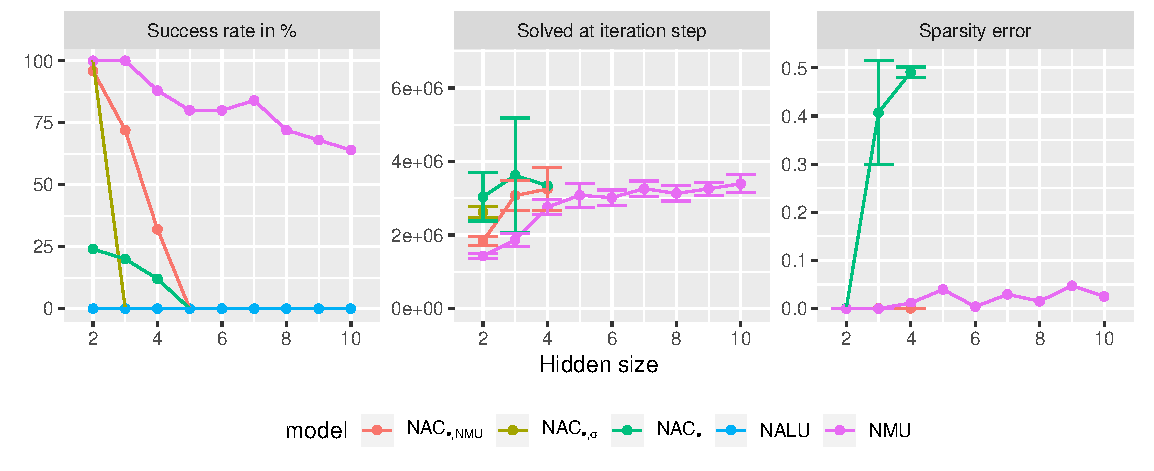
\includegraphics[width=\linewidth,trim={0 1.3cm 0 0},clip]{results/simple_function_static_mul_hidden_size.pdf}
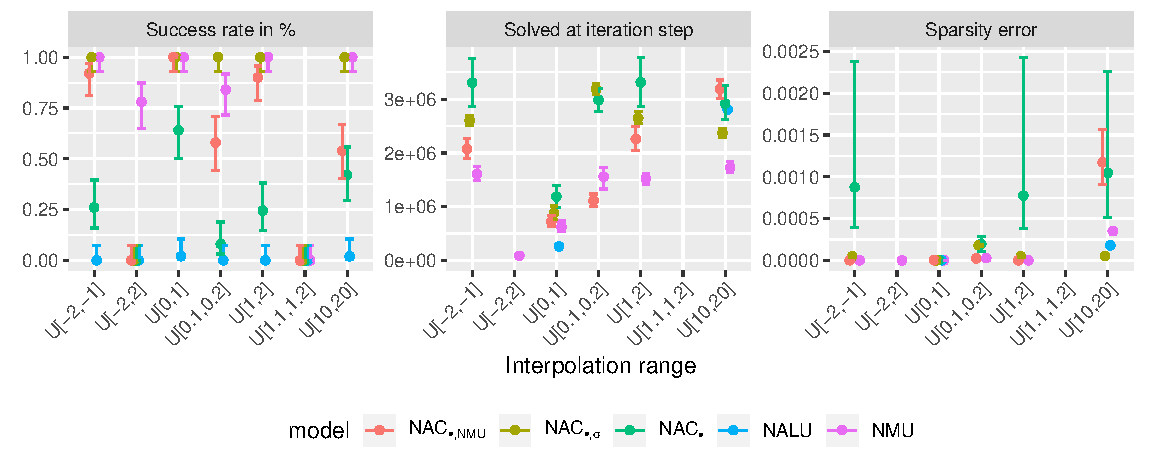
\includegraphics[width=\linewidth,trim={0 0 0 0.809cm},clip]{results/simple_function_static_mul_range.pdf}
\caption{Shows that the NMU can handle a large hidden size, and works when the input contains both positive and negative numbers ($U[-2,-2]$).} 
%\caption{Shows the effect of the dataset parameters. For each interpolation range, the following extrapolation ranges are used: ${\mathrm{U}[-2,2] \rightarrow \mathrm{U}[-6,-2] \cup \mathrm{U}[2,6]}$, ${\mathrm{U}[0,1] \rightarrow \mathrm{U}[1,5]}$, ${\mathrm{U}[0.1,0.2] \rightarrow \mathrm{U}[0.2,2]}$, ${\mathrm{U}[1,2] \rightarrow \mathrm{U}[2,6]}$, ${\mathrm{U}[10, 20] \rightarrow \mathrm{U}[20, 40]}$. The uniform sampling ranges are chosen to test the effect of mean, variance, and sign for optimizing.}
\label{fig:simple-function-static-theoreical-claims-experiment}
\end{figure}

\subsection{Product of sequential MNIST}

To evaluate the NMU's ability to backpropergate though a larger unconstrained neural network, the NMU is applied as a recurrent-unit to a sequence of MNIST digits, where the target is to fit the cumulative product. This task is similar to ``MNIST Counting and Arithmetic Tasks'' in \cite{trask-nalu}, but use multiplication rather than addition, the same CNN model is also used \footnote{\url{https://github.com/pytorch/
examples/tree/master/mnist}}. Each model is trained on sequences of length 2, and then tested on sequences of length 20.

Success of convergence is determined by comparing the MSE of each model, with a baseline model that directly computes the sequential product. If the MSE of each model, is less than the upper 1\% MSE-confidence-interval of the baseline model, then the model is considered successfully converged.

Sparsity and ``solved at iteration step'' is determined as described in experiment \ref{sec:arithmetic-dataset}. The validation set, is the last 5000 MNIST digits from the training set, which is used to select the best epoch.

In this experiment we discovered that having an unconstrained ``input-network'' causes the multiplication-units to learn an undesired solution, such as $(0.1 \cdot 81 + 1 - 0.1) = 9$. This solves the problem with a similar success-rate, but not in the intended way. To prevent such solution, we regularize the CNN output with $\mathcal{R}_{\mathrm{z}} = \frac{1}{H_{\ell-1} H_\ell} \sum_{h_\ell}^{H_\ell} \sum_{h_{\ell-1}}^{H_{\ell-1}} (1 - W_{h_{\ell-1},h_\ell}) \cdot (1 - \bar{z}_{h_{\ell-1}})^2$. This regularizer is applied to the NMU and $\mathrm{NAC}_{\bullet,\mathrm{NMU}}$ models. See appendix \ref{} for the results, when this regularizer is not used.

Figure \ref{fig:sequential-mnist-prod-results} shows that the NMU does not hindre learning a more complex neural network. And that it can extrapolate to much longer sequences than what is is trained on.

\begin{figure}[h]
\centering
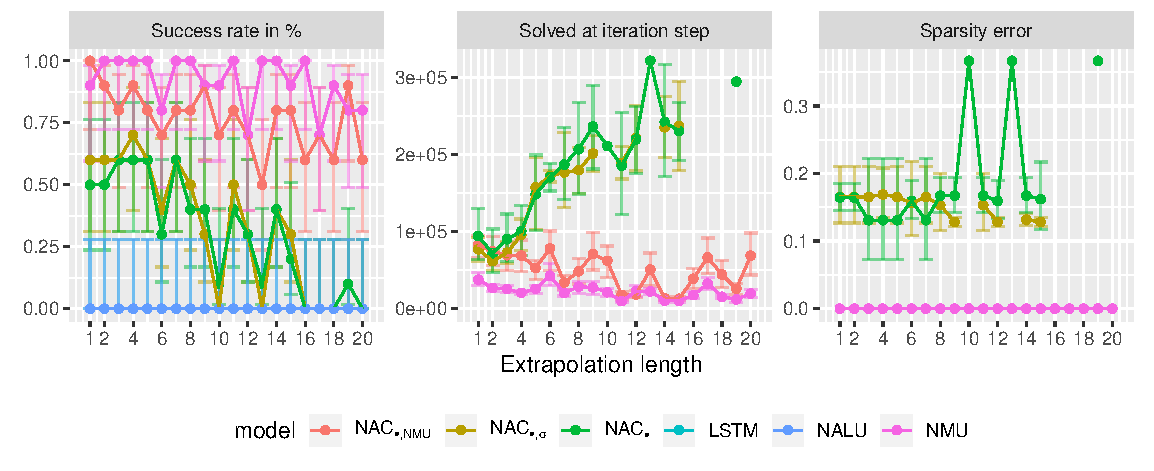
\includegraphics[width=\linewidth,trim={0 0.5cm 0 0},clip]{results/sequential_mnist_prod_long.pdf}
\caption{Shows the ability of each model to backpropergation and extrapolate to larger sequence lengths.} 
\label{fig:sequential-mnist-prod-results}
\end{figure}
